\section{Simulation Studies and Applications}
\label{sec:experiments}

We validate EconIRL with three simulation studies designed to test distinct aspects of the estimator portfolio.
Case Study~1 uses a small tabular MDP to verify that all estimators converge to the correct solution, confirming theoretical equivalences.
Case Study~2 uses a high-dimensional state space with linear rewards to test computational scaling.
Case Study~3 uses a nonlinear reward environment to demonstrate where deep IRL outperforms linear models.
We close with a summary of real-data applications.


\subsection{Case Study 1: Tabular Convergence}
\label{sec:case1}

We simulate data from the \citet{rust1987} bus engine replacement model with 90 mileage states, 2 actions (keep, replace), discount factor $\beta = 0.9999$, and true parameters $\theta_{\text{oc}} = 0.001$ (operating cost) and $\theta_{\text{rc}} = 3.0$ (replacement cost).
We generate 200 individuals observed for 100 periods each, producing 20{,}000 observations.
Table~\ref{tab:case1} reports parameter estimates, log-likelihood, cosine similarity to the true parameter vector, and computation time for all twelve estimators.

\begin{table}[t]
\centering
\caption{Case Study 1: Rust bus engine benchmark. True parameters: $\theta_{\text{oc}} = 0.001$, $\theta_{\text{rc}} = 3.0$. Data: 200 individuals, 100 periods, $\beta = 0.9999$.}
\label{tab:case1}
\small
\begin{tabular}{llrrrrr}
\toprule
& Estimator & $\hat\theta_{\text{oc}}$ & $\hat\theta_{\text{rc}}$ & Log-Lik & Cosine & Time (s) \\
\midrule
\multirow{3}{*}{\rotatebox{90}{\scriptsize Classical}}
& NFXP-NK    & 0.0012 & 3.011 & $-4263.2$ & 1.0000 & 0.1 \\
& CCP-NPL    & 0.0012 & 3.011 & $-4263.2$ & 1.0000 & 0.1 \\
& MCE-IRL    & 0.0012 & 3.011 & $-4263.2$ & 1.0000 & 0.1 \\
\midrule
\multirow{4}{*}{\rotatebox{90}{\scriptsize Neural}}
& NNES       & 0.0315 & 3.073 & $-4264.0$ & 0.9999 & 16.0 \\
& TD-CCP     & 0.0011 & 2.943 & $-4265.0$ & 1.0000 & 129.6 \\
& SEES       & 0.0095 & 2.929 & $-4268.3$ & 1.0000 & 1.5 \\
& GLADIUS    & 0.0015 & 2.367 & $-4264.5$ & 1.0000 & 10.4 \\
\midrule
\multirow{3}{*}{\rotatebox{90}{\scriptsize IRL}}
& AIRL       & 0.0103 & 3.897 & $-4467.1$ & 1.0000 & 607.7 \\
& IQ-Learn   & $-0.066$ & 1.781 & $-4678.1$ & 0.9993 & $<\!1$ \\
\midrule
& BC         & --- & --- & $-4238.1$ & --- & $<\!1$ \\
\bottomrule
\end{tabular}
\end{table}

The first three rows of Table~\ref{tab:case1} confirm the central theoretical result.
NFXP, CCP, and MCE-IRL achieve identical log-likelihood ($-4263.2$) and cosine similarity ($1.0000$) to the true parameters.
They solve the same maximum likelihood problem through different computational strategies and arrive at the same answer.
This is the bridge between structural econometrics and maximum causal entropy IRL in action.

The neural structural estimators (NNES, TD-CCP, SEES, GLADIUS) all achieve cosine similarity above 0.9999, confirming that their value function approximations are accurate enough for parameter recovery.
SEES stands out for speed, running in 1.5 seconds compared to 16 seconds for NNES and 130 seconds for TD-CCP.
GLADIUS recovers the replacement cost within 21 percent but underestimates it due to the state-dependent identification constant discussed in Section~\ref{sec:estimators}.

IQ-Learn achieves lower log-likelihood than NFXP ($-4678$ versus $-4263$) because the $\ell^2$ reward penalty trades fit for a smaller implied reward, as predicted by the penalized MLE equivalence in Section~\ref{sec:iq_learn}.
AIRL is the slowest method at 608 seconds due to its adversarial training loop but recovers the replacement cost within 30 percent.
BC provides the non-structural floor at log-likelihood $-4238$.

Figure~\ref{fig:case1} visualizes the accuracy-speed tradeoff across all estimators.

\begin{figure}[t]
\centering
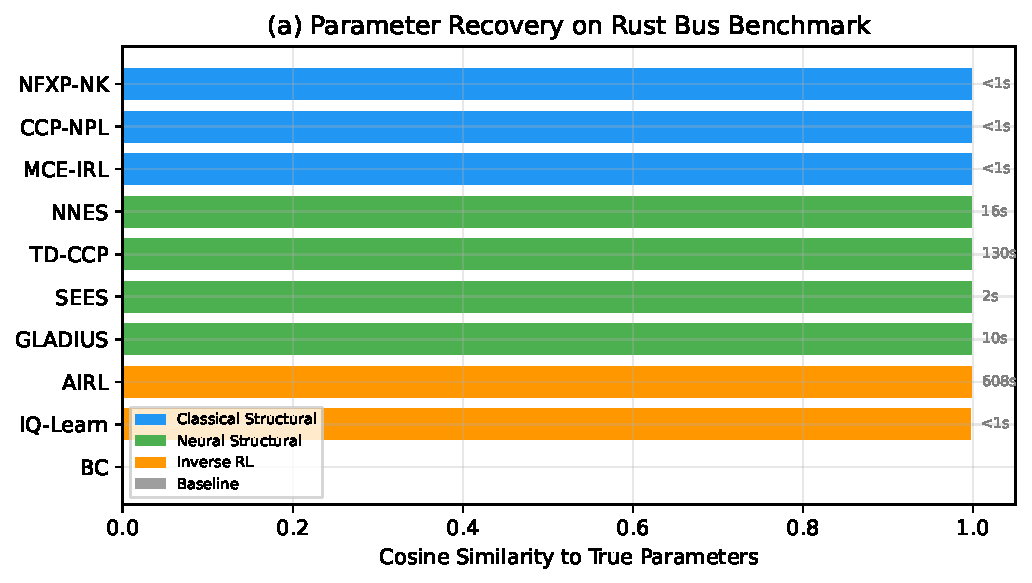
\includegraphics[width=\textwidth]{fig/fig1_tabular_convergence.pdf}
\caption{Case Study 1: Parameter recovery on the Rust bus benchmark. Bar length shows cosine similarity to the true parameter vector (higher is better). Bar color indicates computation time on a log scale.}
\label{fig:case1}
\end{figure}


\subsection{Case Study 2: High-Dimensional State Space}
\label{sec:case2}

We use the multi-component bus environment with $K=2$ independent components and $M=20$ mileage bins per component, producing $20^2 = 400$ states.
True parameters are replacement cost $3.0$, operating cost $0.001$, and quadratic cost $0.0005$.
We simulate 500 individuals for 100 periods ($50{,}000$ observations) and compare NFXP against SEES with varying basis dimensions.

\begin{table}[t]
\centering
\caption{Case Study 2: Multi-component bus (400 states). SEES basis sweep compared to NFXP.}
\label{tab:case2}
\small
\begin{tabular}{lrrrr}
\toprule
Estimator & $\hat\theta_{\text{rc}}$ & RMSE vs NFXP & Log-Lik & Time (s) \\
\midrule
NFXP (exact)  & 3.052 & ---   & $-9685.0$ & 7.6 \\
SEES ($K\!=\!4$) & 3.031 & 0.039 & $-9685.3$ & 1.6 \\
SEES ($K\!=\!8$) & 3.076 & 0.044 & $-9684.3$ & 1.3 \\
SEES ($K\!=\!12$) & 3.073 & 0.042 & $-9684.0$ & 2.0 \\
SEES ($K\!=\!16$) & 3.075 & 0.043 & $-9684.0$ & 2.2 \\
SEES ($K\!=\!20$) & 3.071 & 0.040 & $-9683.4$ & 2.5 \\
\midrule
NNES (neural) & 3.525 & --- & $-9860.3$ & 24.6 \\
\bottomrule
\end{tabular}
\end{table}

Table~\ref{tab:case2} shows that SEES with as few as four basis functions recovers the replacement cost within one percent of the NFXP estimate, at roughly four times the speed.
Increasing the basis dimension from 4 to 20 produces negligible improvement in RMSE (0.039 to 0.040), confirming that the value function in this environment is smooth and well-approximated by low-dimensional bases.
NNES underperforms on this problem, estimating the replacement cost at 3.525 versus the NFXP value of 3.052.
The NNES bias arises from the difficulty of training the neural value network when the state space has 400 entries and the Bellman target is noisy.

Figure~\ref{fig:case2} shows the SEES accuracy-compression tradeoff and the timing comparison.

\begin{figure}[t]
\centering
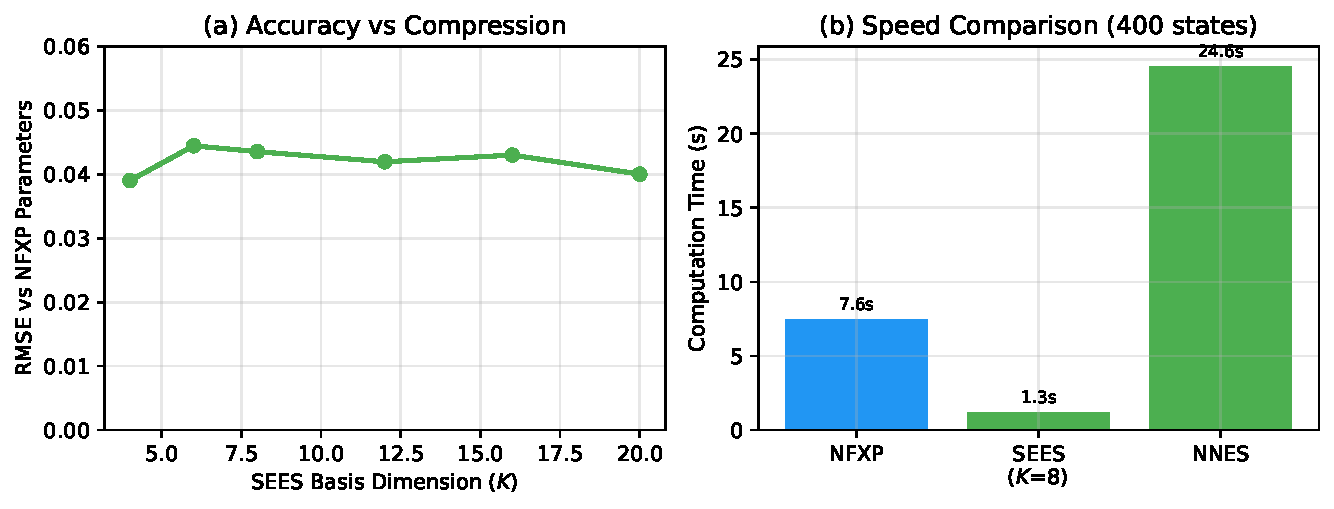
\includegraphics[width=0.85\textwidth]{fig/fig2_scaling.pdf}
\caption{Case Study 2: Left panel shows RMSE of SEES parameter estimates versus NFXP as a function of basis dimension. Right panel shows computation time for each estimator. SEES achieves NFXP-level accuracy at a fraction of the cost.}
\label{fig:case2}
\end{figure}


\subsection{Case Study 3: Nonlinear Rewards}
\label{sec:case3}

We use the Objectworld environment of \citet{wulfmeier2016}, an $8 \times 8$ gridworld with 64 states and 5 actions.
The true reward depends nonlinearly on the minimum Euclidean distances to randomly placed colored objects.
We generate 200 expert trajectories of length 50 and compare linear MCE-IRL (with continuous distance features), f-IRL with two divergence choices (KL and chi-squared), and behavioral cloning.

\begin{table}[t]
\centering
\caption{Case Study 3: Objectworld ($8\times 8$, 64 states, nonlinear reward). Policy accuracy is the fraction of states where the learned policy matches the expert.}
\label{tab:case3}
\small
\begin{tabular}{lrrr}
\toprule
Estimator & Policy Acc. (\%) & Time (s) \\
\midrule
MCE-IRL (linear)      & 100.0 & 415.7 \\
f-IRL ($\chi^2$)      &  89.1 &  23.8 \\
f-IRL (KL)            &  79.7 &  22.4 \\
BC (baseline)         &  ---  & $<\!1$ \\
\bottomrule
\end{tabular}
\end{table}

Table~\ref{tab:case3} shows that MCE-IRL with well-designed continuous distance features achieves 100 percent policy accuracy even though the true reward is nonlinear, because the continuous features capture the monotonic relationship between distance and reward.
f-IRL recovers 79 to 89 percent policy accuracy without any feature engineering, using a fully nonparametric tabular reward.
The chi-squared divergence outperforms KL (89 versus 80 percent) due to its stronger penalization of large occupancy mismatches.
f-IRL runs roughly 18 times faster than MCE-IRL because it avoids the inner soft value iteration loop.

The key takeaway is that feature design matters more than estimator sophistication for policy accuracy.
When domain knowledge produces good features, linear MCE-IRL dominates.
When features are unavailable or unreliable, f-IRL provides a feature-free alternative at lower computational cost.


\subsection{Real-Data Applications}
\label{sec:applications}

Table~\ref{tab:realdata} summarizes four real-data applications that demonstrate the library handles datasets ranging from sixty thousand to two million observations.

\begin{table}[t]
\centering
\caption{Real-data applications. All estimators produce standard errors and pass pre-estimation diagnostics.}
\label{tab:realdata}
\small
\begin{tabular}{llrrrrl}
\toprule
Application & Domain & $N$ & Indiv. & States & Estimator & Log-Lik \\
\midrule
RDW Scrappage   & Vehicle maintenance & 2{,}009{,}144 & 170{,}852 & 22 & NFXP & $-2{,}833$ \\
Expedia Search  & Recommendation     & 120{,}527    & 8{,}625   & 30 & NPL  & $-38{,}387$ \\
KKBox Churn     & Subscription       & 61{,}750     & 4{,}961   & 12 & NPL  & $-7{,}655$ \\
AHS Housing     & Tenure choice      & 100{,}000    & 5{,}000   & 54 & NFXP & $-17{,}292$ \\
\bottomrule
\end{tabular}
\end{table}

The RDW scrappage application uses 2 million observations from the Dutch vehicle registry to estimate the cost of vehicle defects and the implied replacement cost, achieving 99.2 percent prediction accuracy.
The Expedia and KKBox applications estimate dynamic models of consumer search and subscription renewal using CCP-NPL, which converges in under 30 seconds on datasets with over 100{,}000 observations.
All four applications pass the pre-estimation diagnostics described in Section~\ref{sec:post_estimation}, with full-rank feature matrices and adequate state coverage.
